\documentclass[titlepage,11pt]{article}
\usepackage{comment}
\usepackage{enumitem}
\usepackage{transparent} % Untuk transparansi gambar
\usepackage{listings}
\usepackage{amsmath}
\usepackage{graphicx}
\usepackage[font=small,labelfont=bf]{caption}
\usepackage[bahasa]{babel}
\usepackage{float}
\usepackage{verbatim}
\usepackage{graphicx,tabularx,multirow}
\usepackage{xcolor}
\usepackage[onehalfspacing]{setspace}
\usepackage[
	allcolors=visigrey,
	colorlinks=true,
]{hyperref}
\usepackage[a4paper,left=2cm,right=2cm]{geometry}
% Pengaturan kutipan artikel
\usepackage[style=ieee, backend=biber]{biblatex}
%Code listing style pak akok
\definecolor{codegreen}{rgb}{0,0.6,0}
\definecolor{codegray}{rgb}{0.5,0.5,0.5}
\definecolor{codepurple}{rgb}{0.58,0,0.82}
\definecolor{backcolour}{rgb}{0.95,0.95,0.92}

\usepackage{eso-pic} % Untuk menambahkan elemen ke seluruh halaman

\newcommand\BackgroundPic{
  \put(0,0){
    \parbox[b][\paperheight]{\paperwidth}{
      \vfill
      \centering
      \transparent{0.1}
      \includegraphics[width=0.4\paperwidth,keepaspectratio]{miot.png}
      \vfill
    }
  }
}

\newcommand\BackgroundAllPages{ \AddToShipoutPicture*{\BackgroundPic} }
\newcommand\BackgroundNone{ \ClearShipoutPicture } % hilangkan background

\lstdefinestyle{mystyle}{
	backgroundcolor=\color{backcolour}, commentstyle=\color{codegreen},
	keywordstyle=\color{magenta},
	numberstyle=\small\color{codegray},
	stringstyle=\color{codepurple},
	basicstyle=\ttfamily\footnotesize,
	breakatwhitespace=false,         
	breaklines=true,                 
	captionpos=t,                    
	keepspaces=true,                 
	numbers=left,                    
	numbersep=5pt,                  
	showspaces=false,                
	showstringspaces=false,
	showtabs=false,           
	frame = single,
	tabsize=2
}
\lstset{style=mystyle}

\definecolor{visigrey}{rgb}{.1,.15,.15}
\geometry{top=1cm,bottom=.5cm}
\savegeometry{titlepage}
\geometry{top=2cm,bottom=2cm}
\savegeometry{main}

\def\bspace{\(\qquad\qquad\qquad\)}
\usepackage[T1]{fontenc}
\usepackage[utf8]{inputenc}
\usepackage{tgheros}
\renewcommand*\familydefault{\sfdefault}

\setcounter{tocdepth}{6}

\def\autor{Laboratorium }
\def\lab{Multimedia dan Internet of Things}
\def\departemen{Departemen Teknik Komputer}
\def\institut{Institut Teknologi Sepuluh Nopember}
\def\praktikum{Laporan Sementara \\ Praktikum Jaringan Komputer}
\def\nama{Muhammad Zidane Faiq Sidqi - 5024231040}
% Ubah Judul sesuai dengan modul
\def\judul{Jaringan Wireless}
\def\tanggal{2025}
\begin{document}
% Ubah Bahasa sesuai dengan keinginan
\selectlanguage{bahasa}

\BackgroundNone
\def\headingtype{\bf \small}
\loadgeometry{titlepage}

\begin{titlepage}
	\centering
	\begin{tabularx}{\textwidth}{l@{\hskip 0pt}lX}
		\raisebox{-0.5\height}{
\includegraphics[width=3cm]{Cover/img/logodepart.png}} 
		& \raisebox{-0.5\height}{\includegraphics[width=3cm]{Cover/img/miot.png}} 
		& \raggedleft
	\hfill
	\begin{minipage}{0.5\textwidth}
		\raggedleft
		{\emph{\headingtype \autor}} \\[-2pt]
		{\headingtype \lab} \\[-2pt]
		{\headingtype \departemen} \\[-2pt]
		{\headingtype \emph{\institut}}
	\end{minipage}

	\vspace{5cm}
	\end{tabularx}
	
	\vspace{5cm}
	{\Huge \bf \praktikum \par}
	
	\vspace{2cm}
	{\LARGE \bf \judul \par}
	
	\vspace{2cm}
	{\Large \nama \par}
	
	\vfill
	{\Large \tanggal \par}
	
	\vfill
	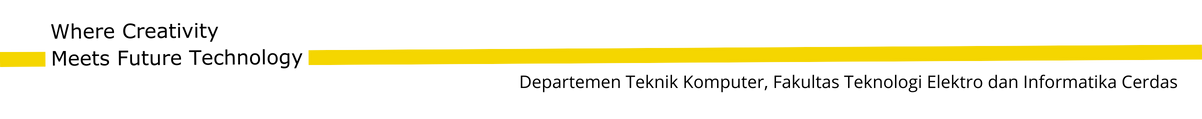
\includegraphics[width=\textwidth]{Cover/img/footer.png}
\end{titlepage}

\loadgeometry{main}


\BackgroundAllPages
% Pilih Modul yang akan di build
\section{Langkah-Langkah Percobaan}
\subsection{Wireless Point-to-Point}
\begin{enumerate}
	\item Melakukan reset pada router jika diperlukan
	\item Mengaktifkan dan mengatur interface wireless wlan1. Untuk router A menggunakan konfigurasi mode bridge dan SSID diberi nama PointToPoint\_17. Untuk router B menggunakan konfigurasi mode station dan melakukan scan lalu memilih SSID dari router A.
	\begin{figure}[H]
		\centering
		\begin{subfigure}[b]{0.4\linewidth}
			\centering
			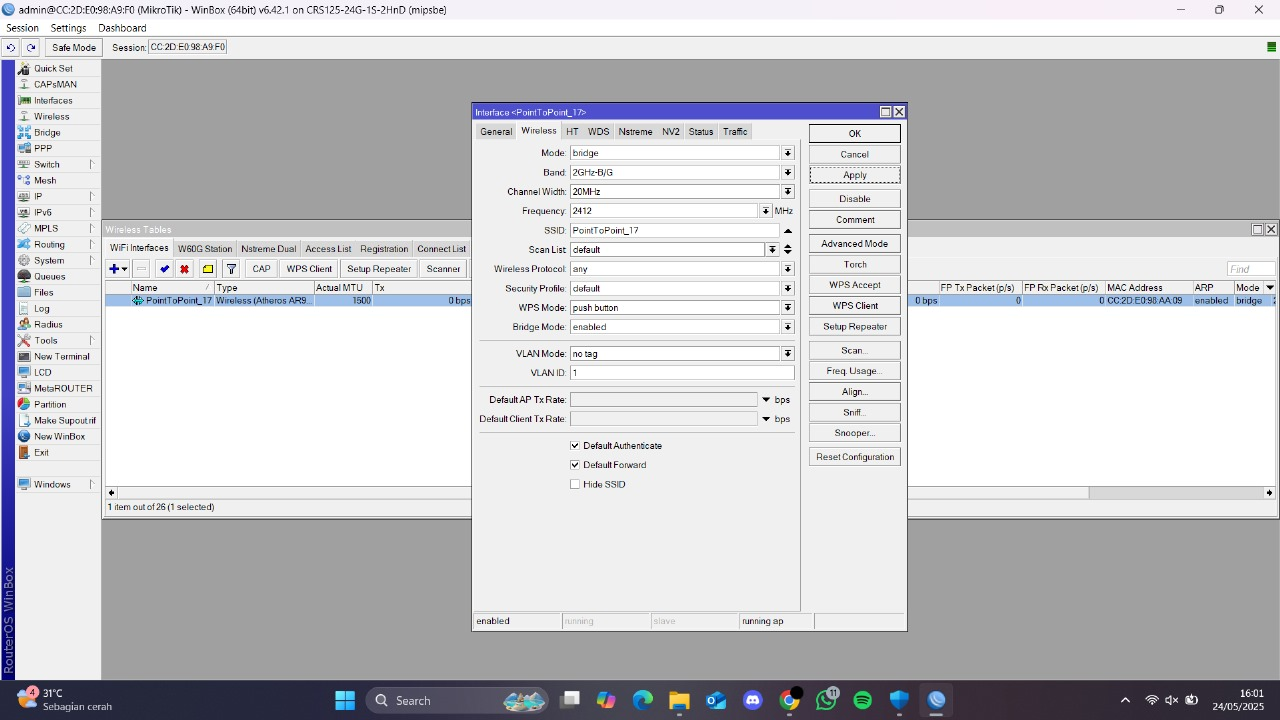
\includegraphics[width=\linewidth]{P3/img/ptp rtrA 1.jpg}
			\caption{Konfigurasi wireless router A\label{fig:konfigurasiR1}}
		\end{subfigure}
		\begin{subfigure}[b]{0.4\linewidth}
			\centering
			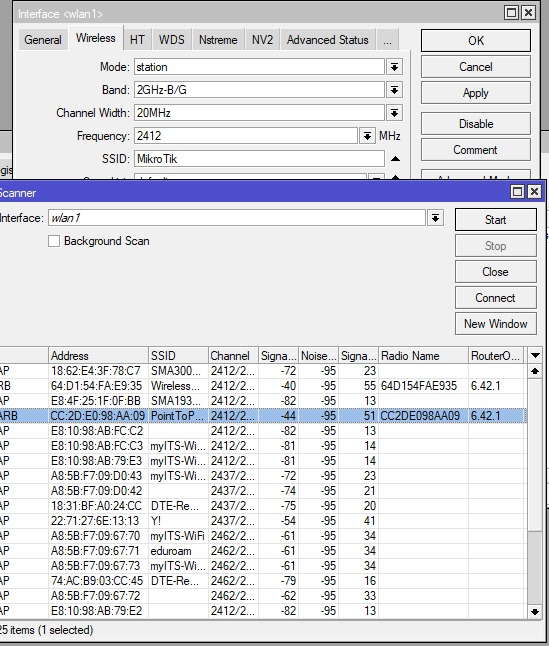
\includegraphics[width=\linewidth]{P3/img/ptp rtrB 1.jpg}
			\caption{Konfigurasi wireless router B\label{fig:konfigurasiR2}}
		\end{subfigure}
		\caption{Konfigurasi wireless router point-to-point}
		\hspace{1cm}
	\end{figure}
	\item Melakukan konfigurasi IP address interface wlan1 untuk koneksi antar router. Pada router A menggunakan alamat IP 10.10.10.1/29 dan pada router B menggunakan alamat IP 10.10.10.2/29
	\item Melakukan konfigurasi IP address pada interface ether1 router A dengan alamat IP 192.168.20.1/24 dan pada interface ether2 router B dengan alamat IP 192.168.30.1/24.
	\item Melakukan konfigurasi routing statis. Pada router A, ditambahkan konfigurasi routing untuk destination address 192.168.30.0/24 dan gateway 10.10.10.2. Pada router B, ditambahkan konfigurasi routing untuk destination address 192.168.20.0/24 dan gateway 10.10.10.1.
	\item Melakukan ping antar router menggunakan wlan1. Pada router A melakukan ping ke 10.10.10.2 dan pada router B melakukan ping ke 10.10.10.1.
	\item Melakukan konfigurasi IP pada laptop. Untuk laptop yang terhubung ke router A menggunakan konfigurasi IP address 192.168.20.2, gateway 102.168.20.1, dan DNS 8.8.8.8. Untuk laptop yang terhubung ke router B menggunakan konfigurasi IP address 192.168.30.2, gateway 102.168.30.1, dan DNS 8.8.8.8.
	\item Melakukan ping antar laptop. Laptop A melakukan ping ke IP laptop B dan sebaliknya.
\end{enumerate}
\subsection{Wireles Point-to-Multipoint}
\begin{enumerate}
	\item Melakukan reset pada router jika diperlukan
	\item Mengaktifkan dan mengatur interface wireless wlan1. Untuk router A menggunakan konfigurasi mode AP bridge dan SSID diberi nama PointToMultipoint\_17. Untuk router B menggunakan konfigurasi mode AP station dan melakukan scan lalu memilih SSID dari router A.
	\begin{figure}[H]
		\centering
		\begin{subfigure}[b]{0.4\linewidth}
			\centering
			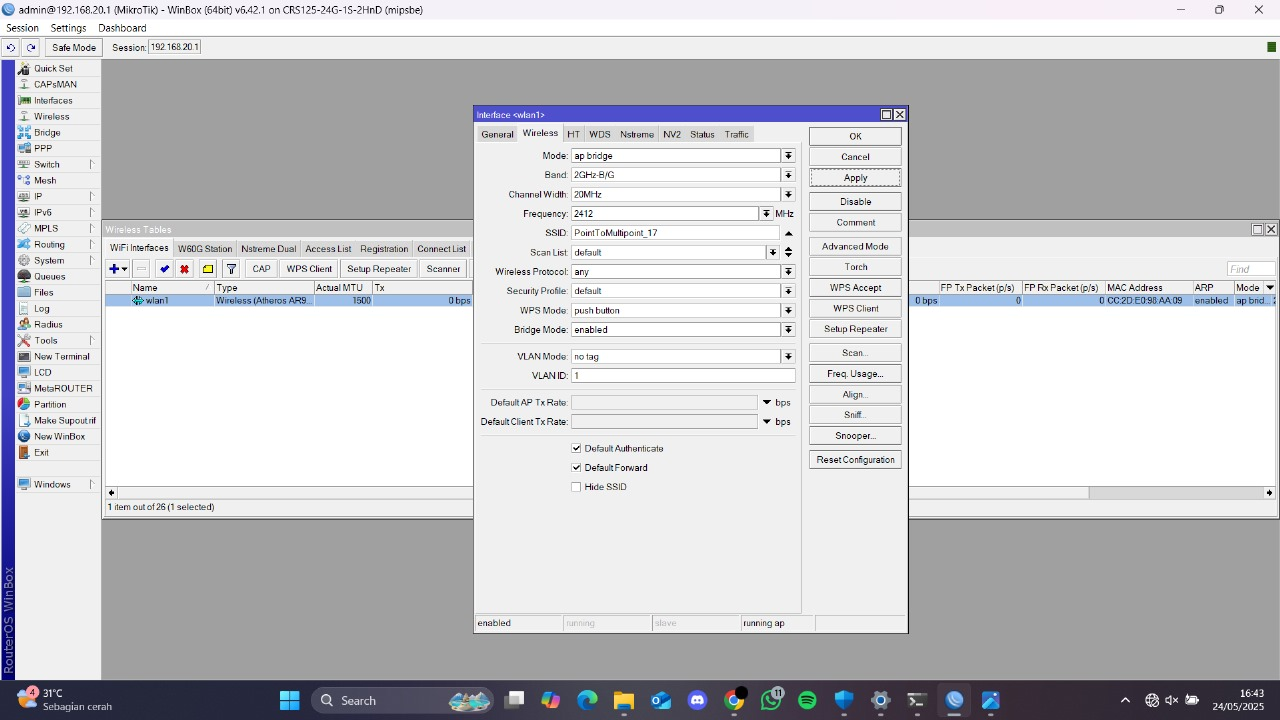
\includegraphics[width=\linewidth]{P3/img/pmp rtrA 1.jpg}
			\caption{Konfigurasi wireless router A\label{fig:konfigurasiR1}}
		\end{subfigure}
		\begin{subfigure}[b]{0.4\linewidth}
			\centering
			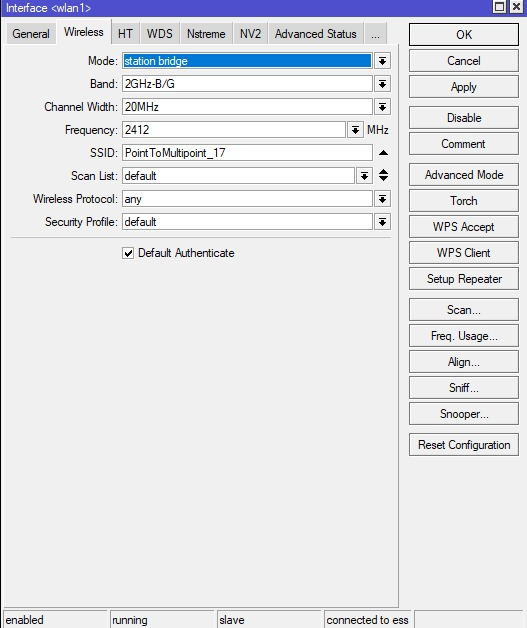
\includegraphics[width=\linewidth]{P3/img/pmp rtrB 1.jpg}
			\caption{Konfigurasi wireless router B\label{fig:konfigurasiR2}}
		\end{subfigure}
		\caption{Konfigurasi wireless router point-to-multipoint}
		\hspace{1cm}
	\end{figure}
	\item Melakukan konfigurasi IP address interface wlan1 untuk koneksi antar router. Pada router A menggunakan alamat IP 10.10.10.1/29 dan pada router B menggunakan alamat IP 10.10.10.2/29.
	
	\item Melakukan konfigurasi IP address pada interface ether1 router A dengan alamat IP 192.168.20.1/24 dan pada interface ether2 router B dengan alamat IP 192.168.30.1/24.
	\item Melakukan konfigurasi routing statis. Pada router A, ditambahkan konfigurasi routing untuk destination address 192.168.30.0/24 dan gateway 10.10.10.2. Pada router B, ditambahkan konfigurasi routing untuk destination address 192.168.20.0/24 dan gateway 10.10.10.1.
	\item Melakukan ping antar router menggunakan wlan1. Pada router A melakukan ping ke 10.10.10.2 dan pada router B melakukan ping ke 10.10.10.1.
	\item Melakukan konfigurasi IP pada laptop. Untuk laptop yang terhubung ke router A menggunakan konfigurasi IP address 192.168.20.2, gateway 102.168.20.1, dan DNS 8.8.8.8. Untuk laptop yang terhubung ke router B menggunakan konfigurasi IP address 192.168.30.2, gateway 102.168.30.1, dan DNS 8.8.8.8.
	\item Melakukan ping antar laptop. Laptop A melakukan ping ke IP laptop B dan sebaliknya.
\end{enumerate}

\subsection{Wireless Bridge}
\begin{enumerate}
	\item Melakukan reset pada router jika diperlukan
	\item Mengaktifkan dan mengatur interface wireless wlan1. Untuk router A menggunakan konfigurasi mode bridge dan SSID diberi nama WirelessBridge\_17. Untuk router B menggunakan konfigurasi mode station pseudobridge dan melakukan scan lalu memilih SSID dari router A.
	\begin{figure}[H]
		\centering
		\begin{subfigure}[b]{0.4\linewidth}
			\centering
			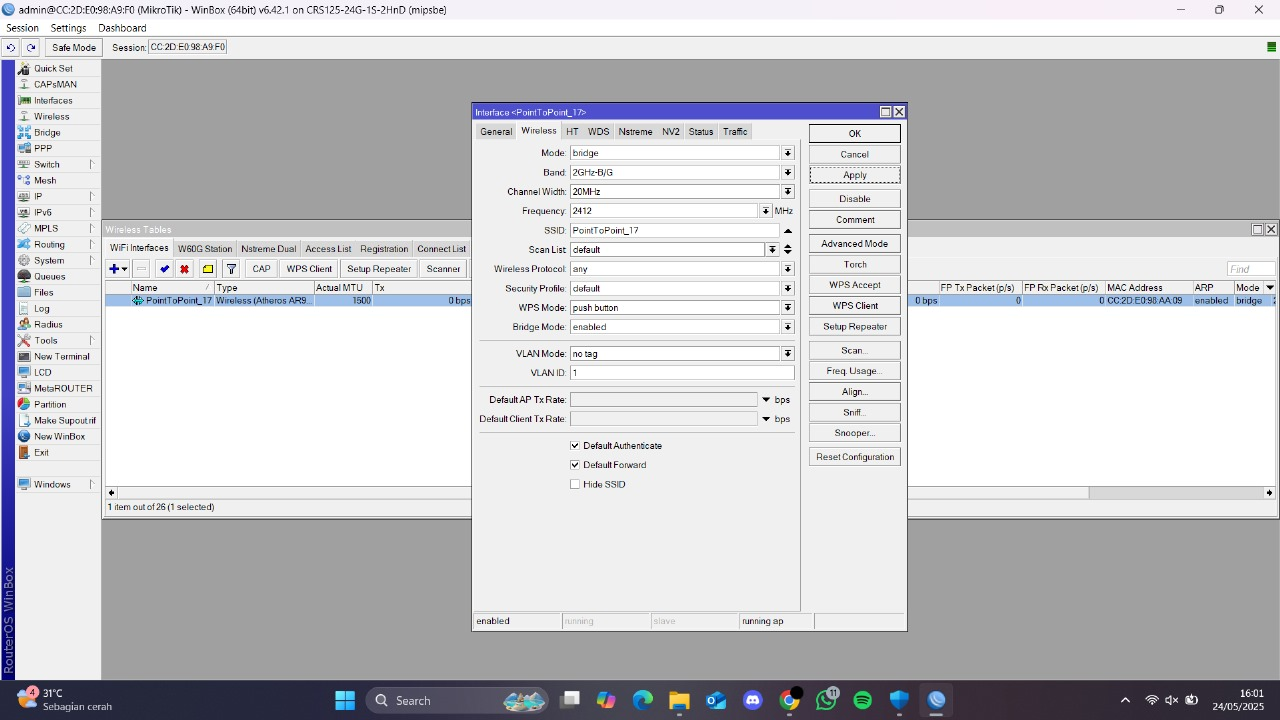
\includegraphics[width=\linewidth]{P3/img/ptp rtrA 1.jpg}
			\caption{Konfigurasi wireless router A\label{fig:konfigurasiR1}}
		\end{subfigure}
		\begin{subfigure}[b]{0.4\linewidth}
			\centering
			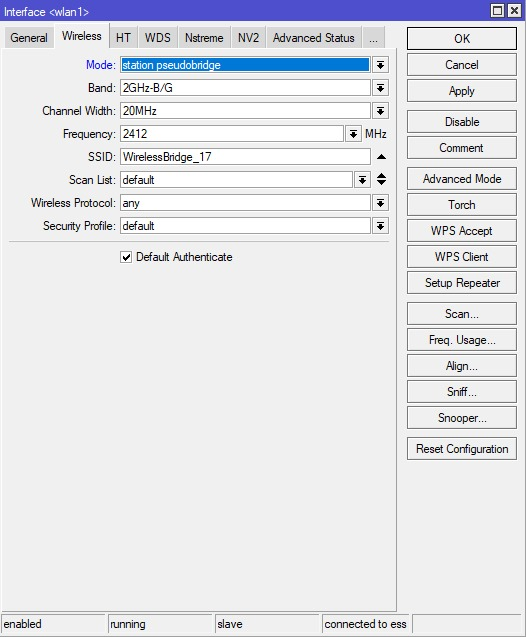
\includegraphics[width=\linewidth]{P3/img/wb rtrB 1.jpg}
			\caption{Konfigurasi wireless router B\label{fig:konfigurasiR2}}
		\end{subfigure}
		\caption{Konfigurasi wireless router wireless  bridge}
		\hspace{1cm}
	\end{figure}
	\item Melakukan konfigurasi IP address interface wlan1 untuk koneksi antar router. Pada router A menggunakan alamat IP 10.10.10.1/29 dan pada router B menggunakan alamat IP 10.10.10.2/29
	\item Melakukan konfigurasi IP address pada interface ether1 router A dengan alamat IP 192.168.10.2/24 dan pada interface ether2 router B dengan alamat IP 192.168.10.3/24.
	\item Melakukan konfigurasi bridge pada router A dan B dengan membuat bridge baru dan melakukan konfigurasi pada interface wlan1 dan ether1 (atau ether2, sesuai dengan interface penghubung ke laptop) menggunakan bridge yang sudah dibuat.
	\begin{figure}[H]
		\centering
		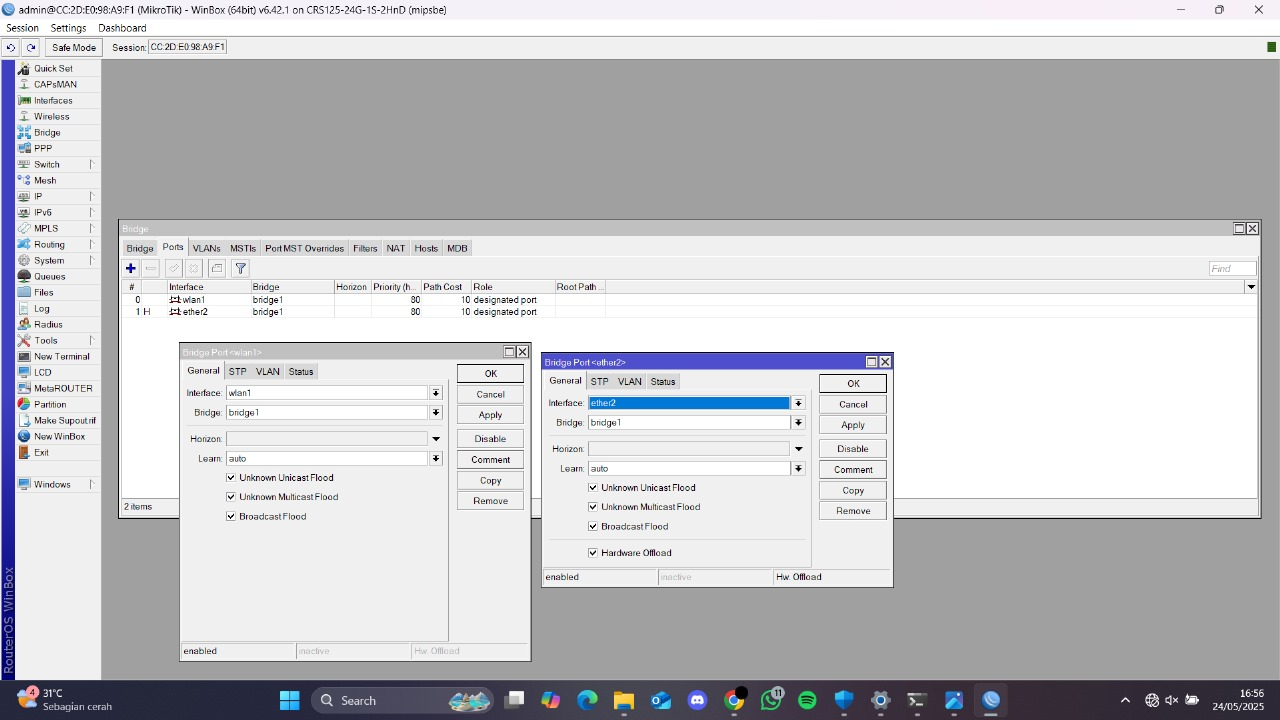
\includegraphics[scale=0.5]{P3/img/wb bridge.jpg}
		\caption{Konfigurasi bridge}
	\end{figure}
	\item Melakukan ping antar router menggunakan wlan1. Pada router A melakukan ping ke 10.10.10.2 dan pada router B melakukan ping ke 10.10.10.1.
	\item Melakukan konfigurasi IP pada laptop. Untuk laptop yang terhubung ke router A menggunakan konfigurasi IP address 192.168.10.5, gateway 102.168.10.2, dan DNS 8.8.8.8. Untuk laptop yang terhubung ke router B menggunakan konfigurasi IP address 192.168.10.7, gateway 102.168.10.3, dan DNS 8.8.8.8.
	\item Melakukan ping antar laptop. Laptop A melakukan ping ke IP laptop B dan sebaliknya.
\end{enumerate}

\section{Analisis Hasil Percobaan}
Pada percobaan pertama, dilakukan percobaan untuk membuat jaringan wireless point-to-point. Jaringan wireless point-to-point digunakan untuk melakukan komunikasi wireless antar router dengan hubungan one to one dengan satu router berperan sebagai bridge (pemancar sinyal wireless) dan satu router beperan sebagai station (penerima sinyal wireless). Pengaturan IP dan routing pada konfigurasi jaringan wireless point-to-point hampir sama dengan konfigurasi IP address dan routing statis pada konfigurasi jaringan berkabel, hanya saja untuk koneksi antar router menggunakan wlan sebagai interface koneksi. Secara teori, bila konfigurasi routing berhasil, maka laptop yang terhubung dengan router dapat melakukan ping satu sama lain meskipun router tidak terhubung secara fisik menggunakan kabel. Menurut hasil yang didapatkan, berhasil dilakukan ping antara laptop A dan laptop B, sehingga membuktikan bahwa teori benar dan praktikum berhasil.
\begin{figure}[H]
	\centering
	\begin{subfigure}[b]{0.4\linewidth}
		\centering
		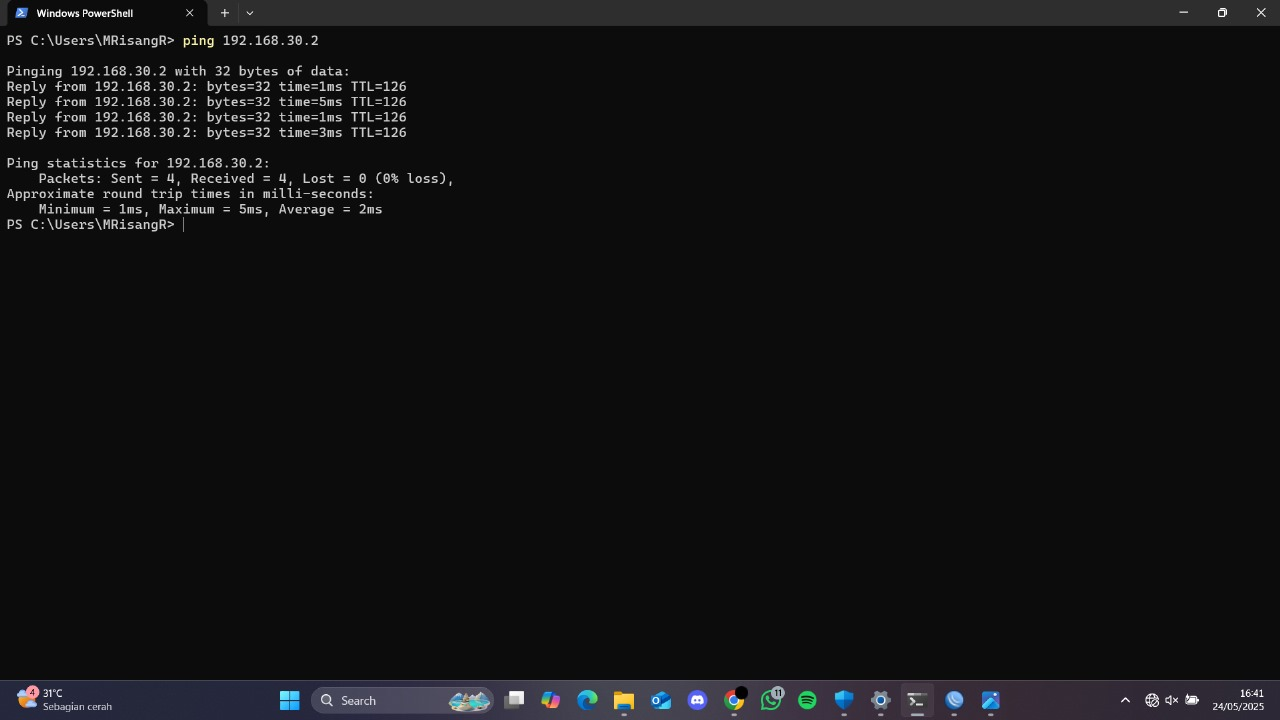
\includegraphics[width=\linewidth]{P3/img/ptp ping a.jpg}
		\caption{Hasil ping laptop A ke laptop B\label{fig:konfigurasiR1}}
	\end{subfigure}
	\begin{subfigure}[b]{0.4\linewidth}
		\centering
		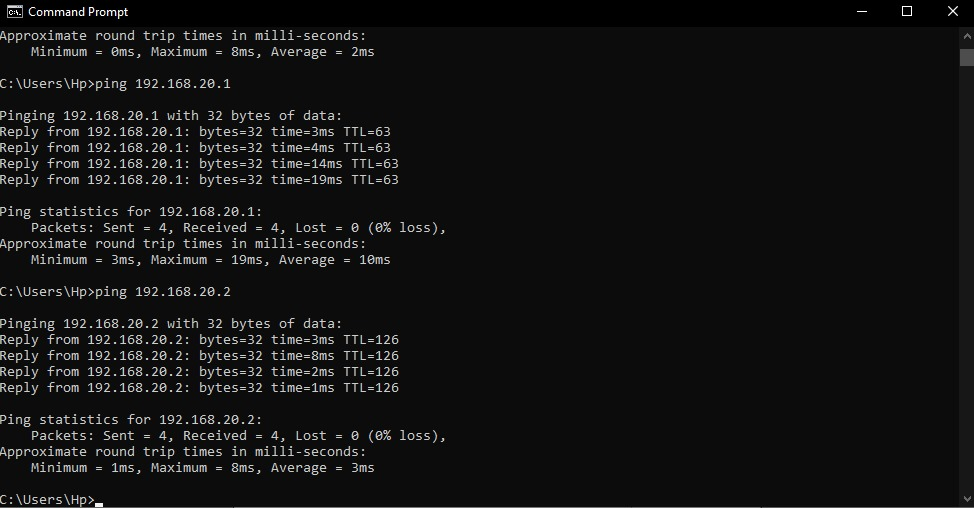
\includegraphics[width=\linewidth]{P3/img/ptp ping b.jpg}
		\caption{Hasil ping laptop B ke laptop A (bagian bawah)\label{fig:konfigurasiR2}}
	\end{subfigure}
	\caption{Konfigurasi wireless router point-to-multipoint}
	\hspace{1cm}
\end{figure}

Pada percobaan kedua, dilakukan percobaan untuk membuat jaringan wireless point-to-multipoint. Jaringan wireless point-to-multipoiny digunakan untuk melakukan komunikasi wireless antar router dengan hubungan one to many dengan satu router berperan sebagai AP bridge dan router lain berperan sebagai AP station. Pengaturan IP dan routing pada konfigurasi jaringan wireless point-to-multipoint hampir sama dengan konfigurasi point-to-point, yang membedakan hanyalah mode wireless yang digunakan pada router. Bila pada point-to-point mode wireless yang digunakan adalah bridge dan station, pada point-to-multipoint mode wireless yang digunakan adalah AP bridge dan AP station. Secara teori, bila konfigurasi routing berhasil maka laptop yang terhubung dengan router dapat melakukan ping satu sama lain dan dalam jaringan dapat terdiri atas beberapa router wireless yang terhubung satu sama lain, namun, dalam praktikum hanya digunakan dua router saja. Menurut hasil yang didapatkan, berhasil dilakukan ping antara laptop A dan laptop B, sehingga membuktikan bahwa teori benar dan praktikum berhasil.
\begin{figure}[H]
	\centering
	\begin{subfigure}[b]{0.4\linewidth}
		\centering
		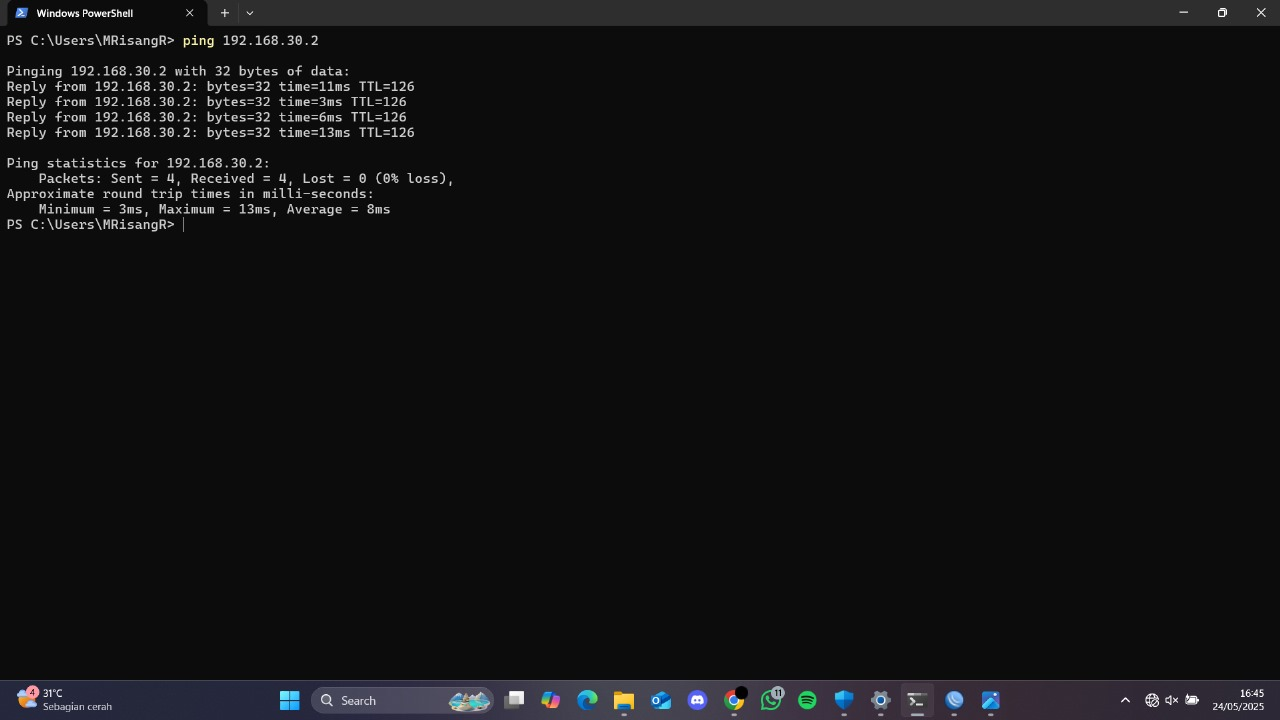
\includegraphics[width=\linewidth]{P3/img/pmp ping a.jpg}
		\caption{Hasil ping laptop A ke laptop B\label{fig:konfigurasiR1}}
	\end{subfigure}
	\begin{subfigure}[b]{0.4\linewidth}
		\centering
		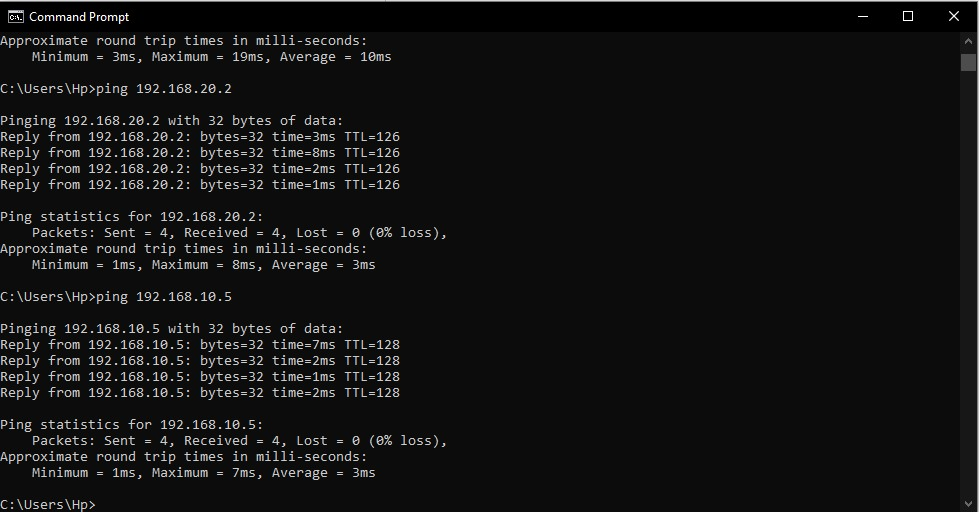
\includegraphics[width=\linewidth]{P3/img/ptp wb ping b.jpg}
		\caption{Hasil ping laptop B ke laptop A (bagian atas)\label{fig:konfigurasiR2}}
	\end{subfigure}
	\caption{Konfigurasi wireless router point-to-multipoint}
	\hspace{1cm}
\end{figure}

Pada percobaan ketiga, dilakukan percobaaan untuk membuat jaringan wireless bridge. Wireless bridge merupakan teknik yang digunakan untuk melakukan ekstensi pada sebuah jaringan wireless dengan menghubungkan router menggunakan bridge. Berbeda dengan metode point-to-point dan point-to-multipoint, wireless bridge juga menghubungkan jaringan LAN antar router, sehingga pada perangkat (dalam hal ini laptop) yang terhubung dengan router dapat memiliki network address yang sama meskipun secara fisik terhubung pada router yang berbeda. Dalam praktikum ini, router difungsikan juga sebagai bridge wireless dan konfigurasi alamat untuk semua perangkat menggunakan network address 192.168.10.0. Secara teori, apabila konfigurasi wireless bridge benar dan berhasil maka seluruh perangkat dalam jaringan dapat melakukan ping ke satu sama lain dengan network address yang sama meskipun terhubung pada router yang berbeda. Menurut hasil yang didapatkan, berhasil dilakukan ping antara laptop A dan laptop B, sehingga membuktikan bahwa teori benar dan praktikum berhasil.
\begin{figure}[H]
	\centering
	\begin{subfigure}[b]{0.4\linewidth}
		\centering
		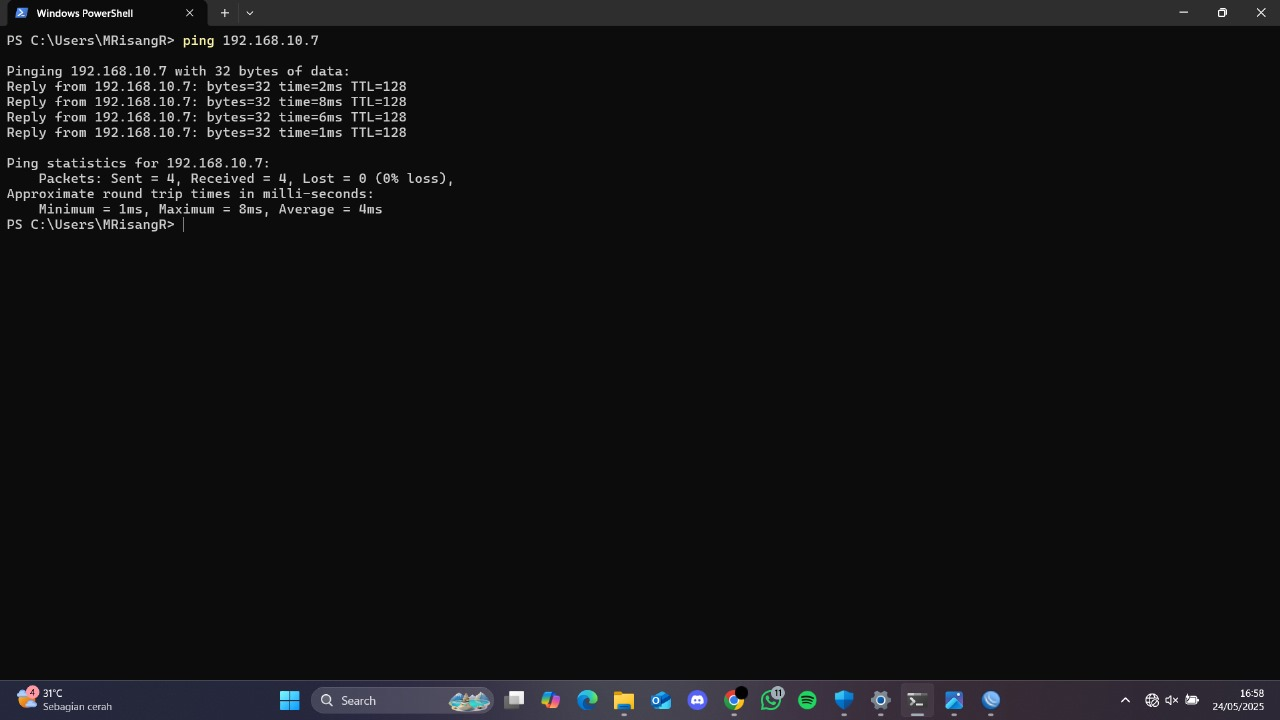
\includegraphics[width=\linewidth]{P3/img/wb ping a.jpg}
		\caption{Hasil ping laptop A ke laptop B\label{fig:konfigurasiR1}}
	\end{subfigure}
	\begin{subfigure}[b]{0.4\linewidth}
		\centering
		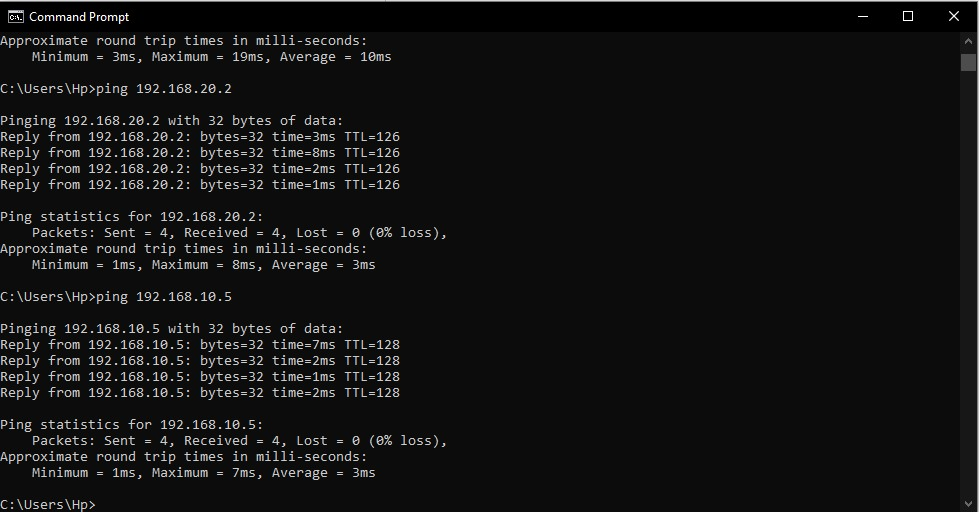
\includegraphics[width=\linewidth]{P3/img/ptp wb ping b.jpg}
		\caption{Hasil ping laptop B ke laptop A (bagian bawah)\label{fig:konfigurasiR2}}
	\end{subfigure}
	\caption{Konfigurasi wireless router point-to-multipoint}
	\hspace{1cm}
\end{figure}

\section{Hasil Tugas Modul}
\begin{enumerate}
	\item Simulasikan jaringan wireless antara tiga gedung:
	Gedung Pusat
	Gedung Lab
	Gedung Asrama (Hubungkan dua bagian dalam Gedung Asrama (Blok A dan Blok B) menggunakan Wireless Bridge Point-to-Point.)
	Menggunakan Point-to-Multipoint (PTMP) di Cisco Packet Tracer.\\
	\begin{figure}[H]
		\centering
		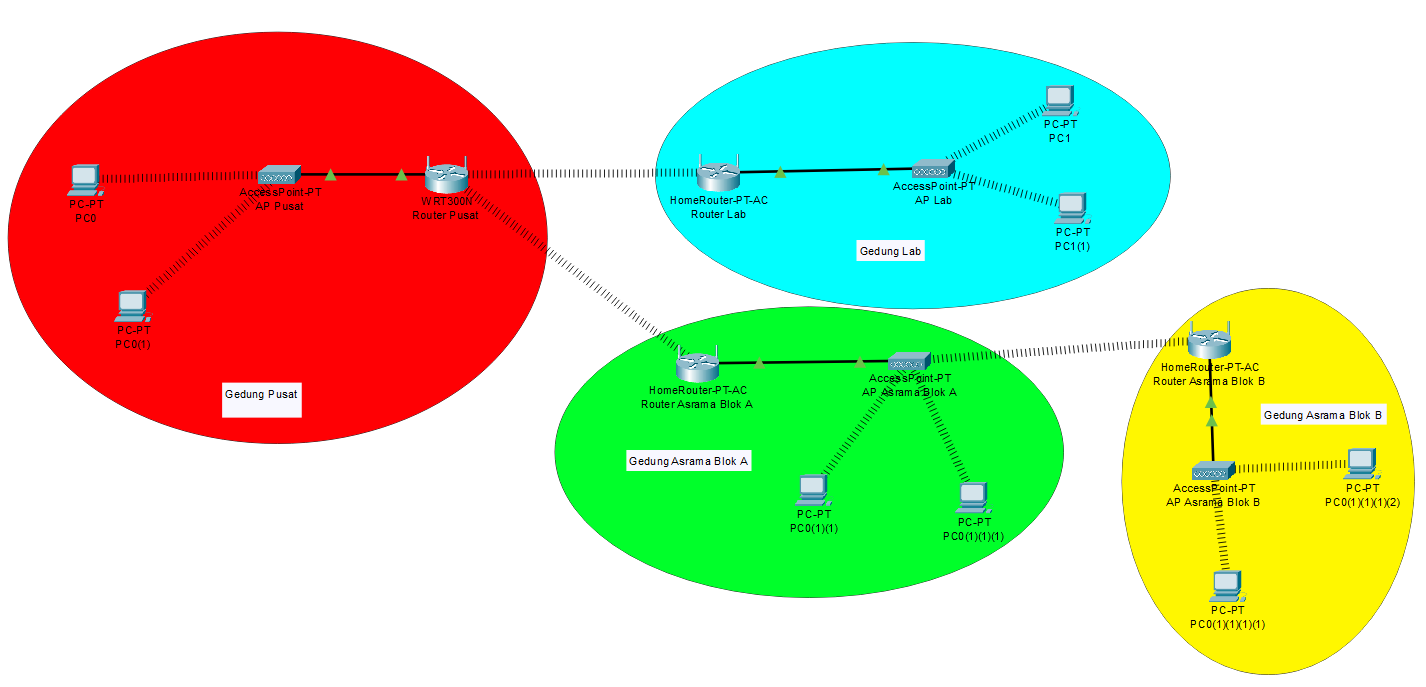
\includegraphics[scale=0.5]{P3/img/tumod.png}
		\caption{Topologi Jaringan}
	\end{figure}
	Di atas merupakan topologi jaringan untuk menghubungkan 3 gedung secara wireless. Router pusat dihubungkan dengan metode wireless bridge multipoint to point ke router gedung asrama blok A dan gedung lab, kemudian router asrama blok A dihubungkan ke access point yang kemudian akan menghubungkan antara jaringan di asrama blok A dengan router asrama blok B.
\end{enumerate}

\section{Kesimpulan}
Melalui praktikum ini, dapat disimpulkan bahwa penggunaan jaringan wireless dalam sebuah sistem jaringan merupakan teknik yang dapat mempermudah pembangunan jaringan karena dengan memanfaatkan jaringan wireless maka jaringan tidak bergantung lagi pada koneksi kabel fisik untuk dapat terhubung. Dari semua percobaan yang dilakukan semua dapat dilakukan dan terbukti benar, sehingga praktikum jaringan komputer modul jaringan wireless dapat disimpulkan berhasil.

\section{Lampiran}
\subsection{Dokumentasi saat praktikum}
\begin{figure}[H]
	\centering
	\begin{subfigure}[b]{0.4\linewidth}
		\centering
		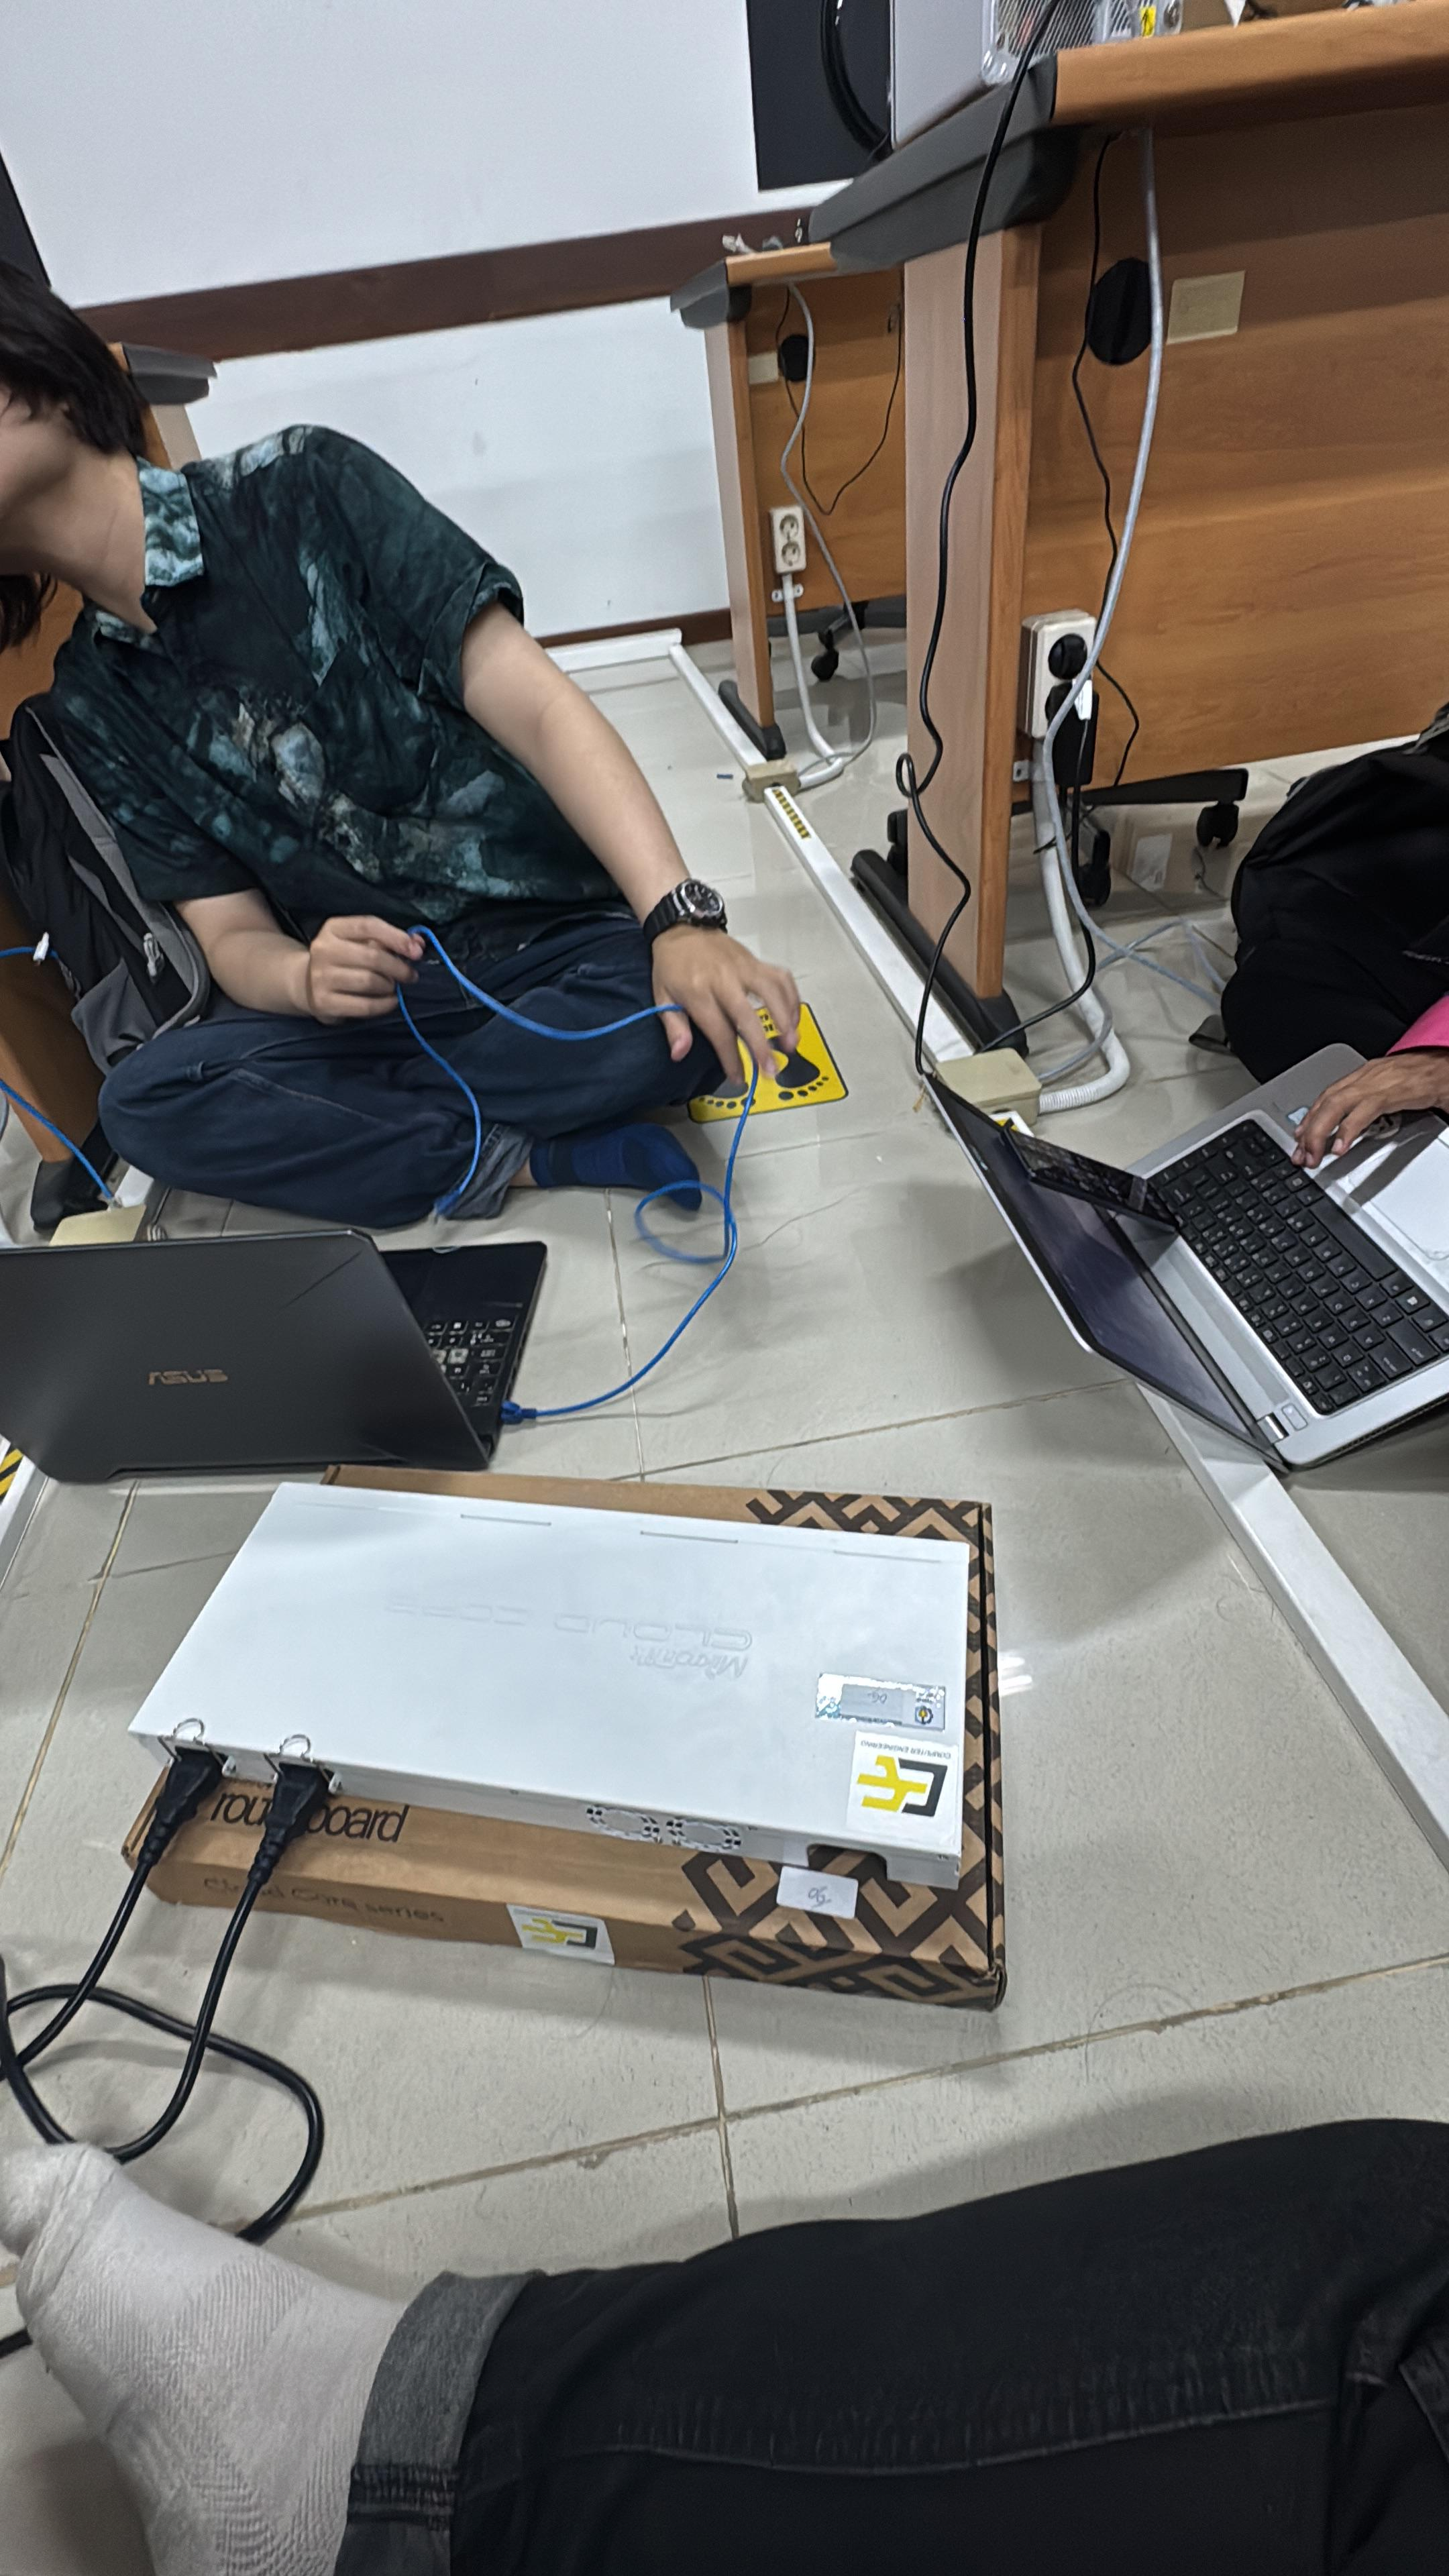
\includegraphics[width=\linewidth]{P3/img/dokum.jpg}
	\end{subfigure}
	\begin{subfigure}[b]{0.4\linewidth}
		\centering
		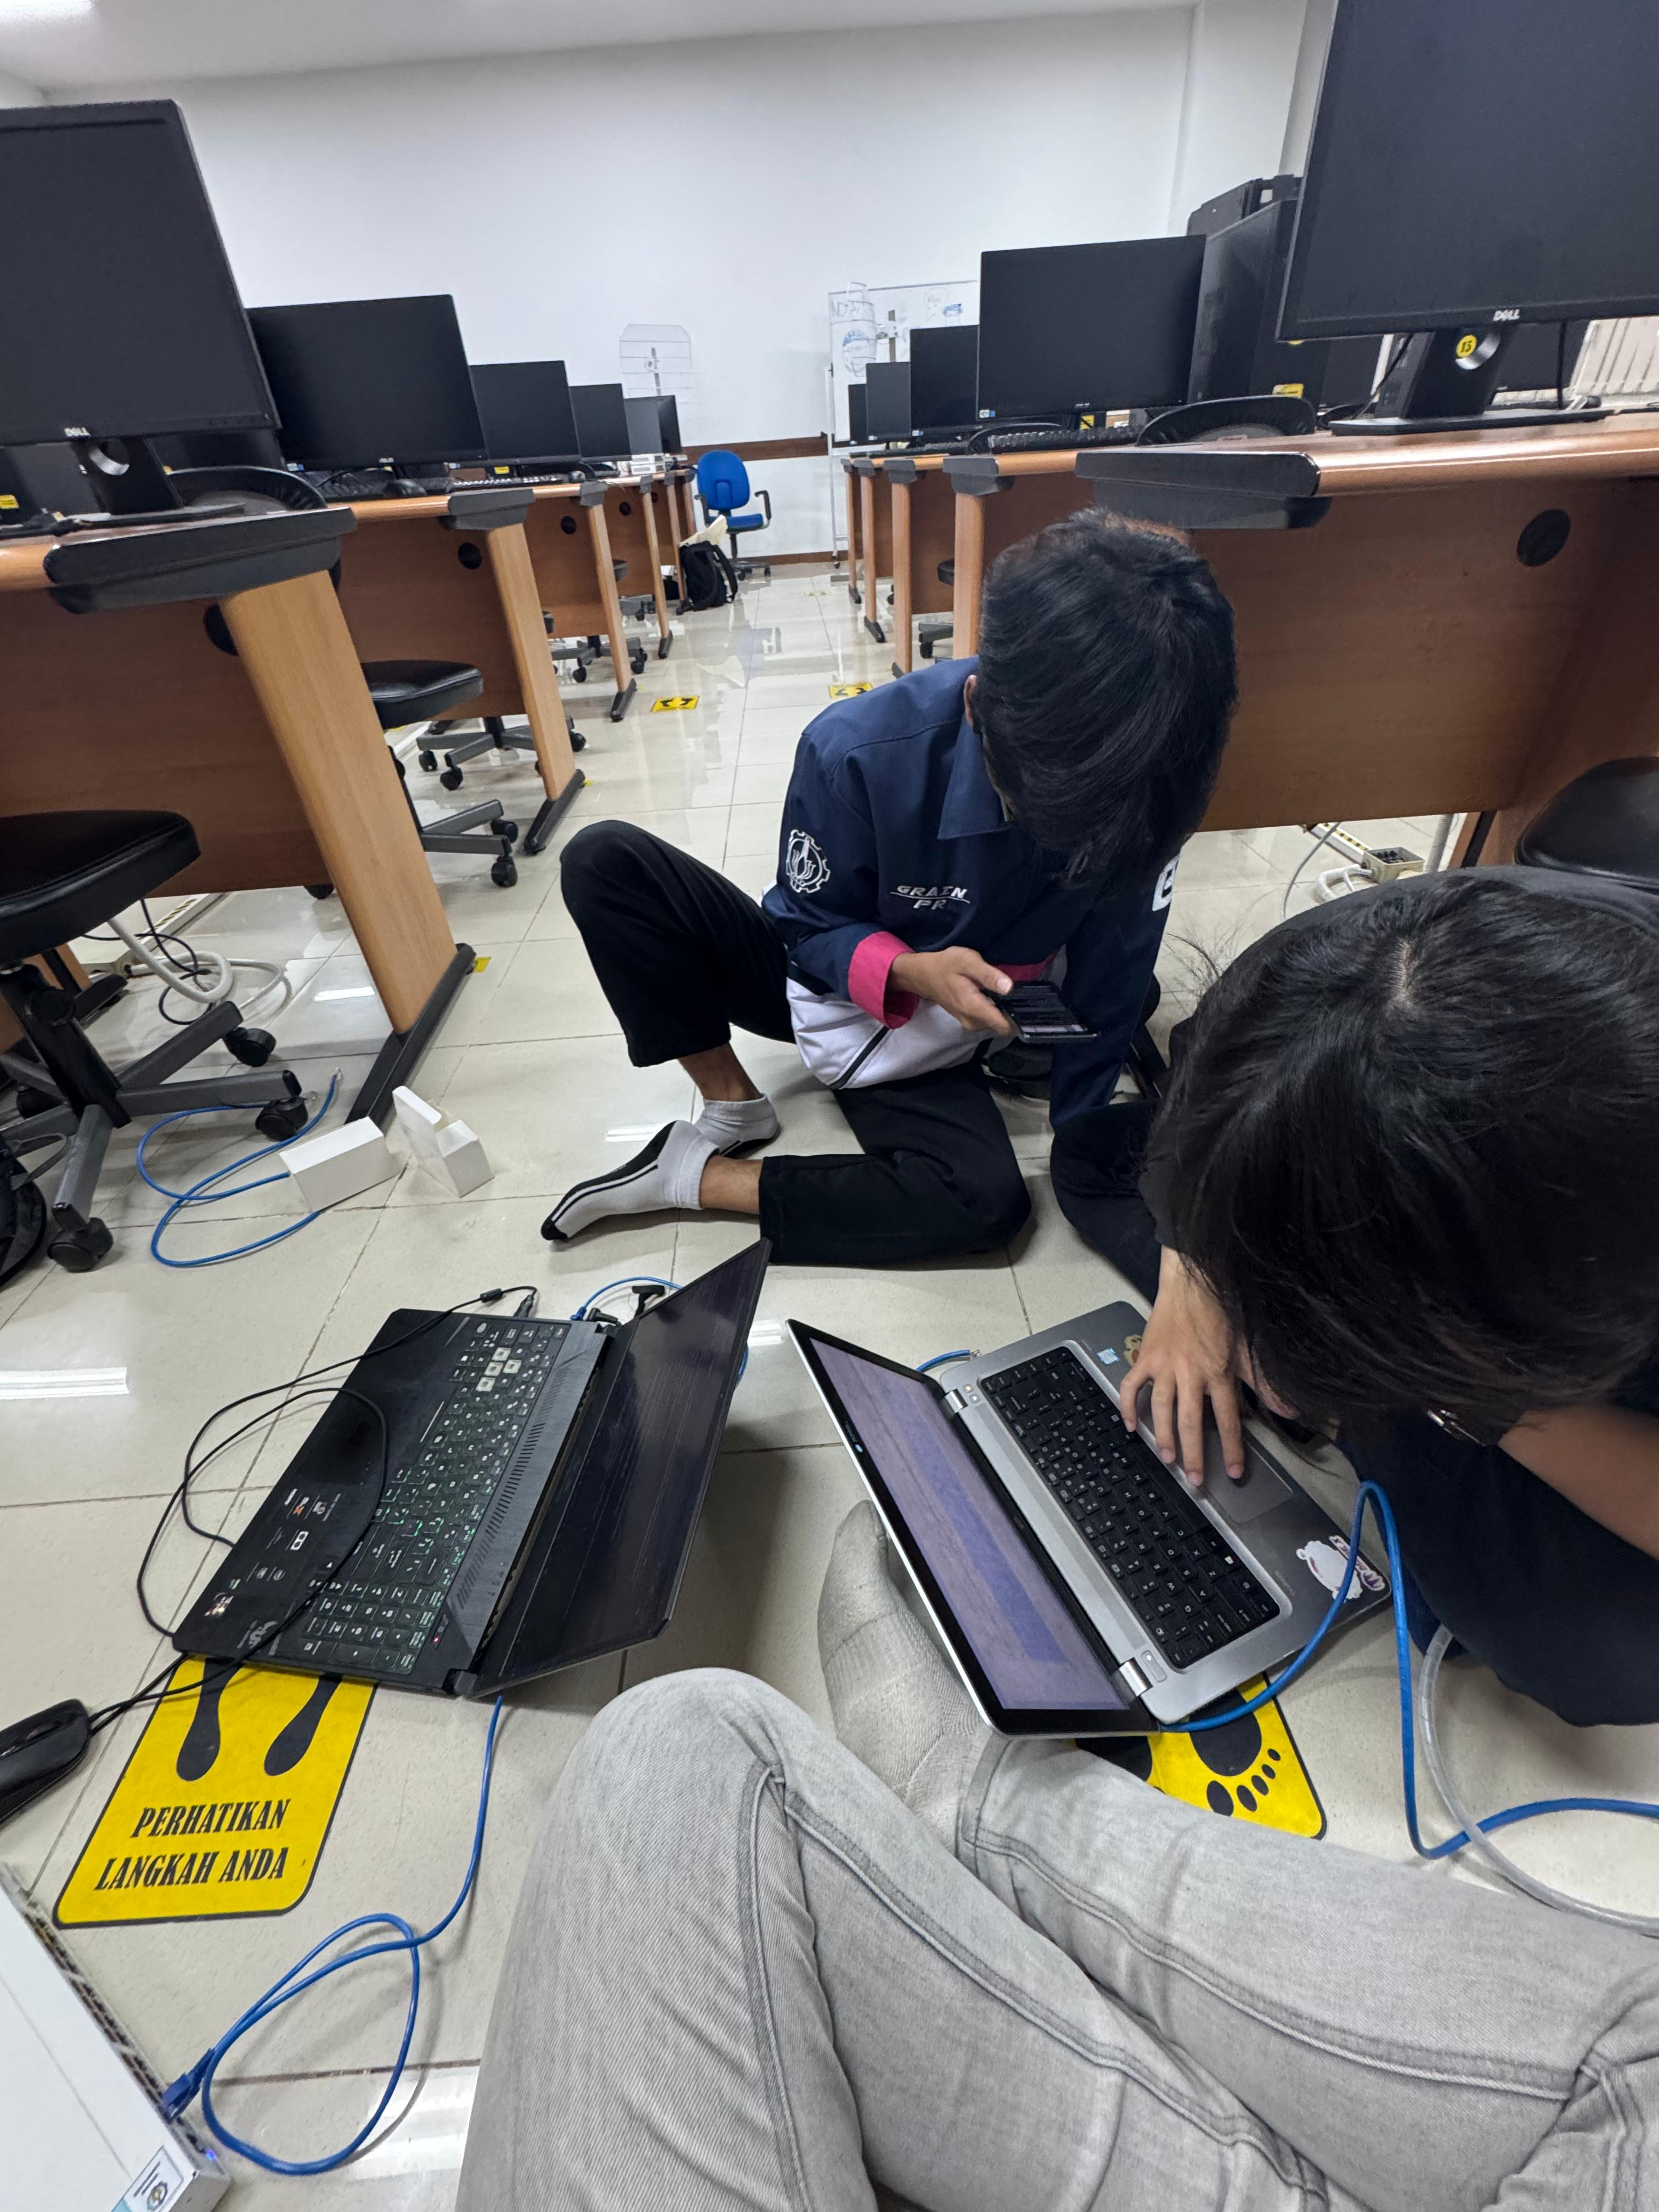
\includegraphics[width=\linewidth]{P3/img/dokum 2.jpg}
	\end{subfigure}
\end{figure}
\begin{figure}[H]
	\centering
	\begin{subfigure}[b]{0.4\linewidth}
		\centering
		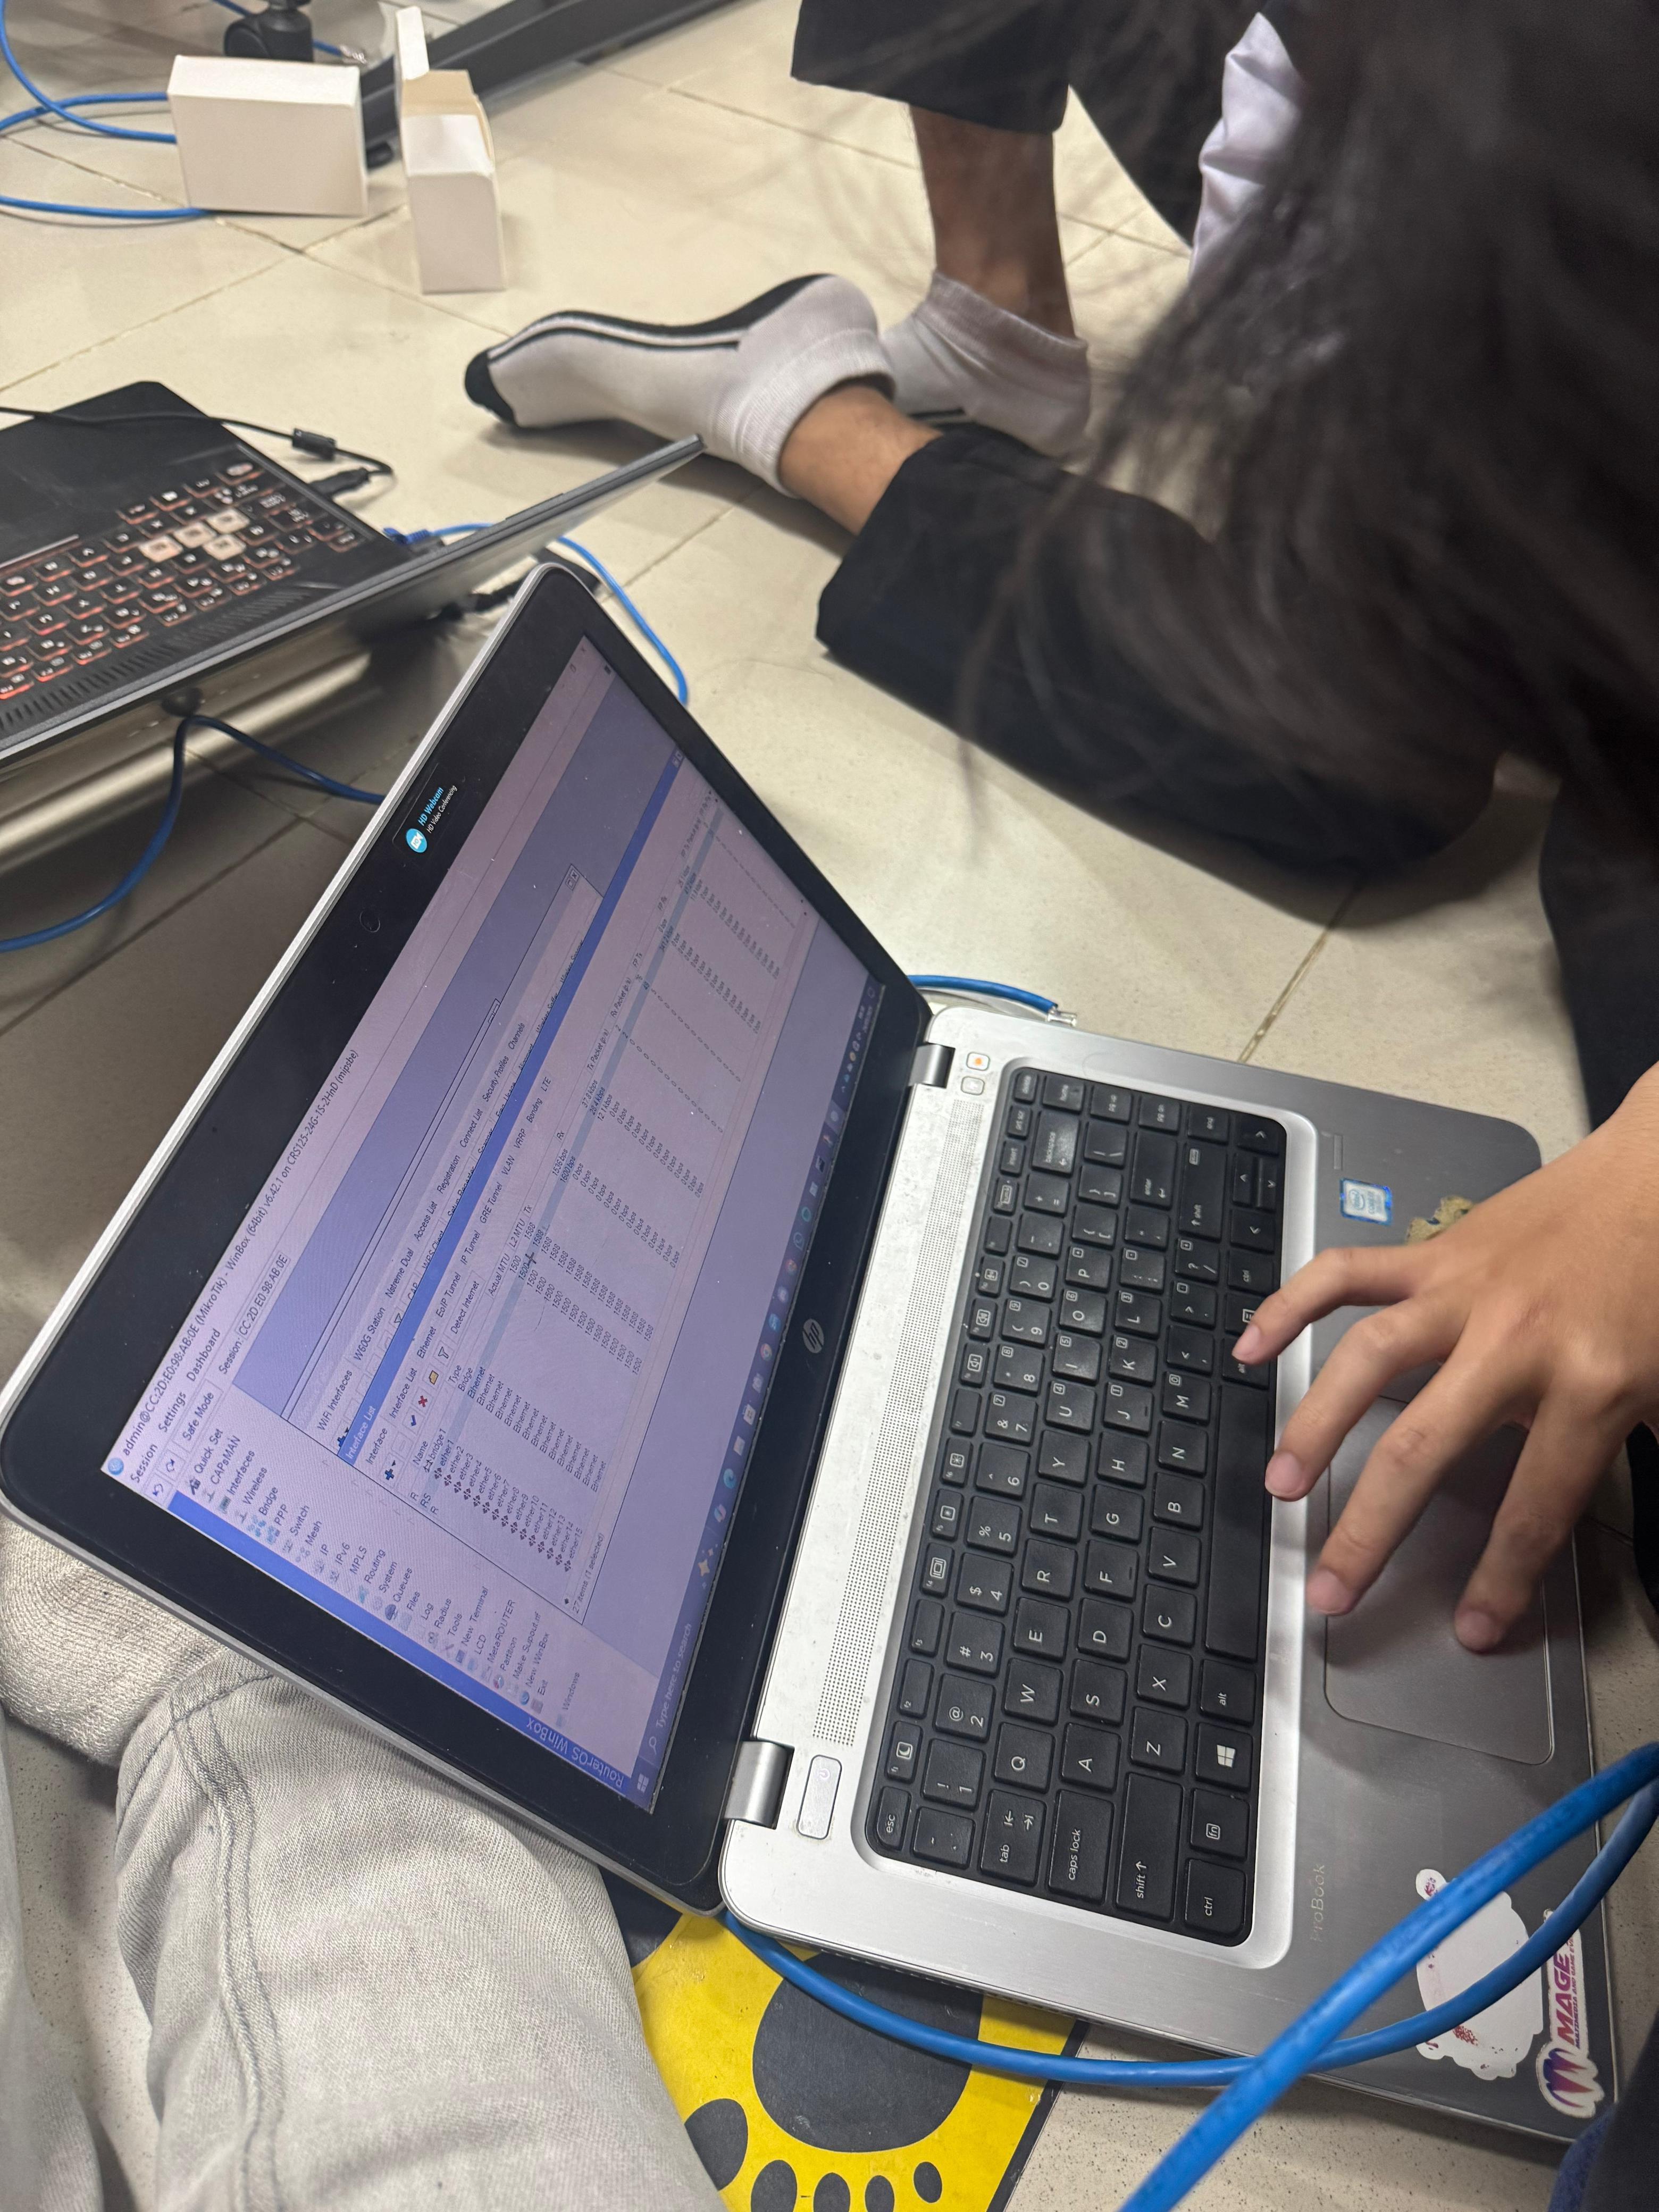
\includegraphics[width=\linewidth]{P3/img/dokum 3.jpg}
	\end{subfigure}
	\begin{subfigure}[b]{0.4\linewidth}
		\centering
		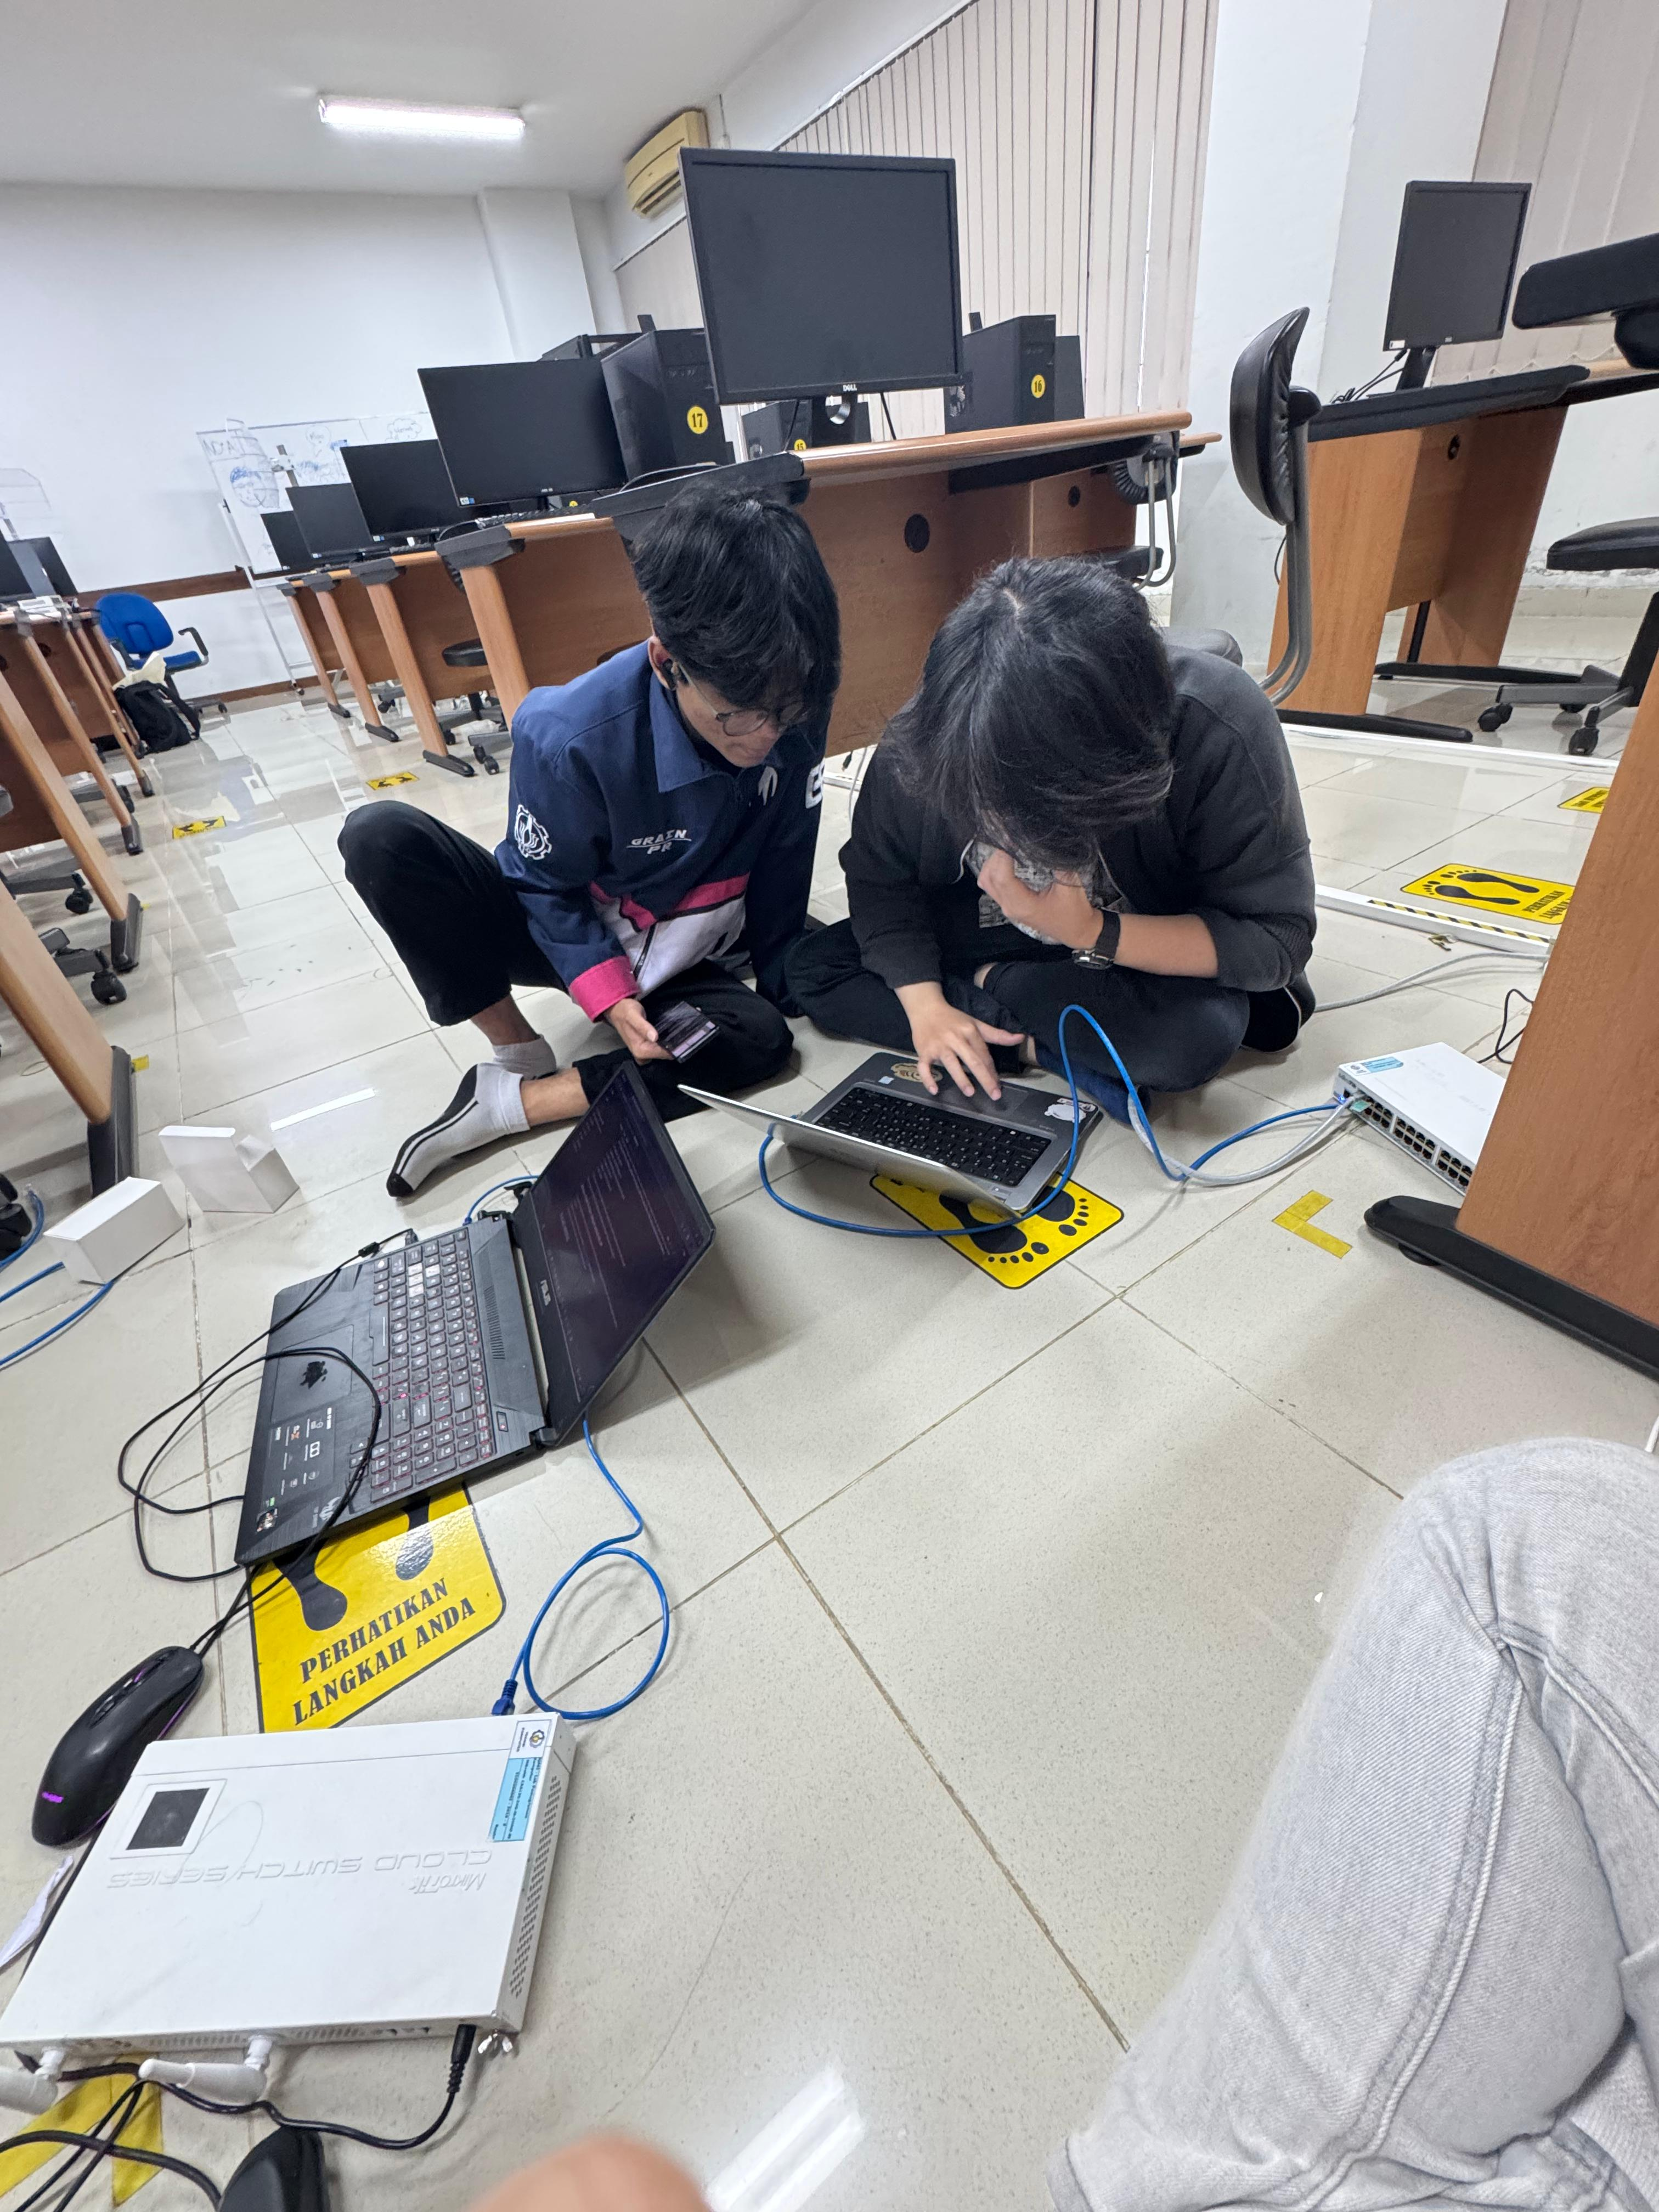
\includegraphics[width=\linewidth]{P3/img/dokum 4.jpg}
	\end{subfigure}
\end{figure}

\end{document}